\section{Evaluation}

For evaluation, we did experiments for both action-noun map and news search engine.

\subsection{Action-noun map evaluation}
The testing action-noun map we use is generated from a news corpus with around 1.7 million
news articles. We managed to extract 4,863 unique action classes that have at least 100 times of mentionings
in the corpus.
For the noun concepts, we used a noun set containing 529 unique nouns that are first extracted from
the testing news corpus, then filtered by Probase, as mentioned in the approach section.

Since there is no existing testing dataset for such task, we created our own dataset and evaluate
our result by letting human judges to label them.
First we chose 50 action classes based on the principal that they should be meaningful, commonsensical, and
conceptualizable in general. Then we present for each of these action classes the top 10 noun concepts from
the action-noun map we generated. We ask human judges to label each noun concept with either positive or negative.
Positive if the noun concept is a good abstraction of the action class, otherwise it should be labeled with negative.

Table 1 shows some of our action-noun map results.
It can be seen from this table that, apart from some good noun abstractions, there are also some noun concepts
that are close to the action class but cannot subsume the majority of the action class.
Example of such kind includes ``wildfire'' for ``event destroy place'', ``birthday'' for ``person
celebrate event''. Since by definition our conceptualization requires the action class to be covered by the noun concept,
we deem such cases together with completely irrelevant nouns as negative while labeling.

First we compute Precision at K(see Figure 1). This represents the number of positive results divided by the number of all test problems,
at cut off K. The precision for top-1 is 32\%, which suggests that about 32\% of the first noun concepts are regarded by human judges as
good abstraction for the correspondent action classes.

We also conducted another test where for each noun returned, if the majority of human judges label the noun
as positive, we say an agreement is reached on this noun and set it to positive, otherwise we set the noun as negative.
And with this agreement data we compute the Average Precision(AP) and Mean Average Precision(MAP). For Average Precision
it measures for each action class the performance of the noun concepts, which is computed by averaging the precision at k
wherever k the recall changes. For example the sequence ``POS,NEG,POS'' would yield an Average Precision value of
$(1 + \frac{2}{3})\times\frac{1}{2}$. Then averaging these AP values will give us a Mean Average Precision value. Our MAP result is 29.85\%,
which is effectively close to returning the right noun at the third place in the action-noun map. And for 29 out of 50 evaluation action classes,
there is at least one positive agreement reached within the top 10 noun results.
\begin{figure}[!htp]
 \centering
 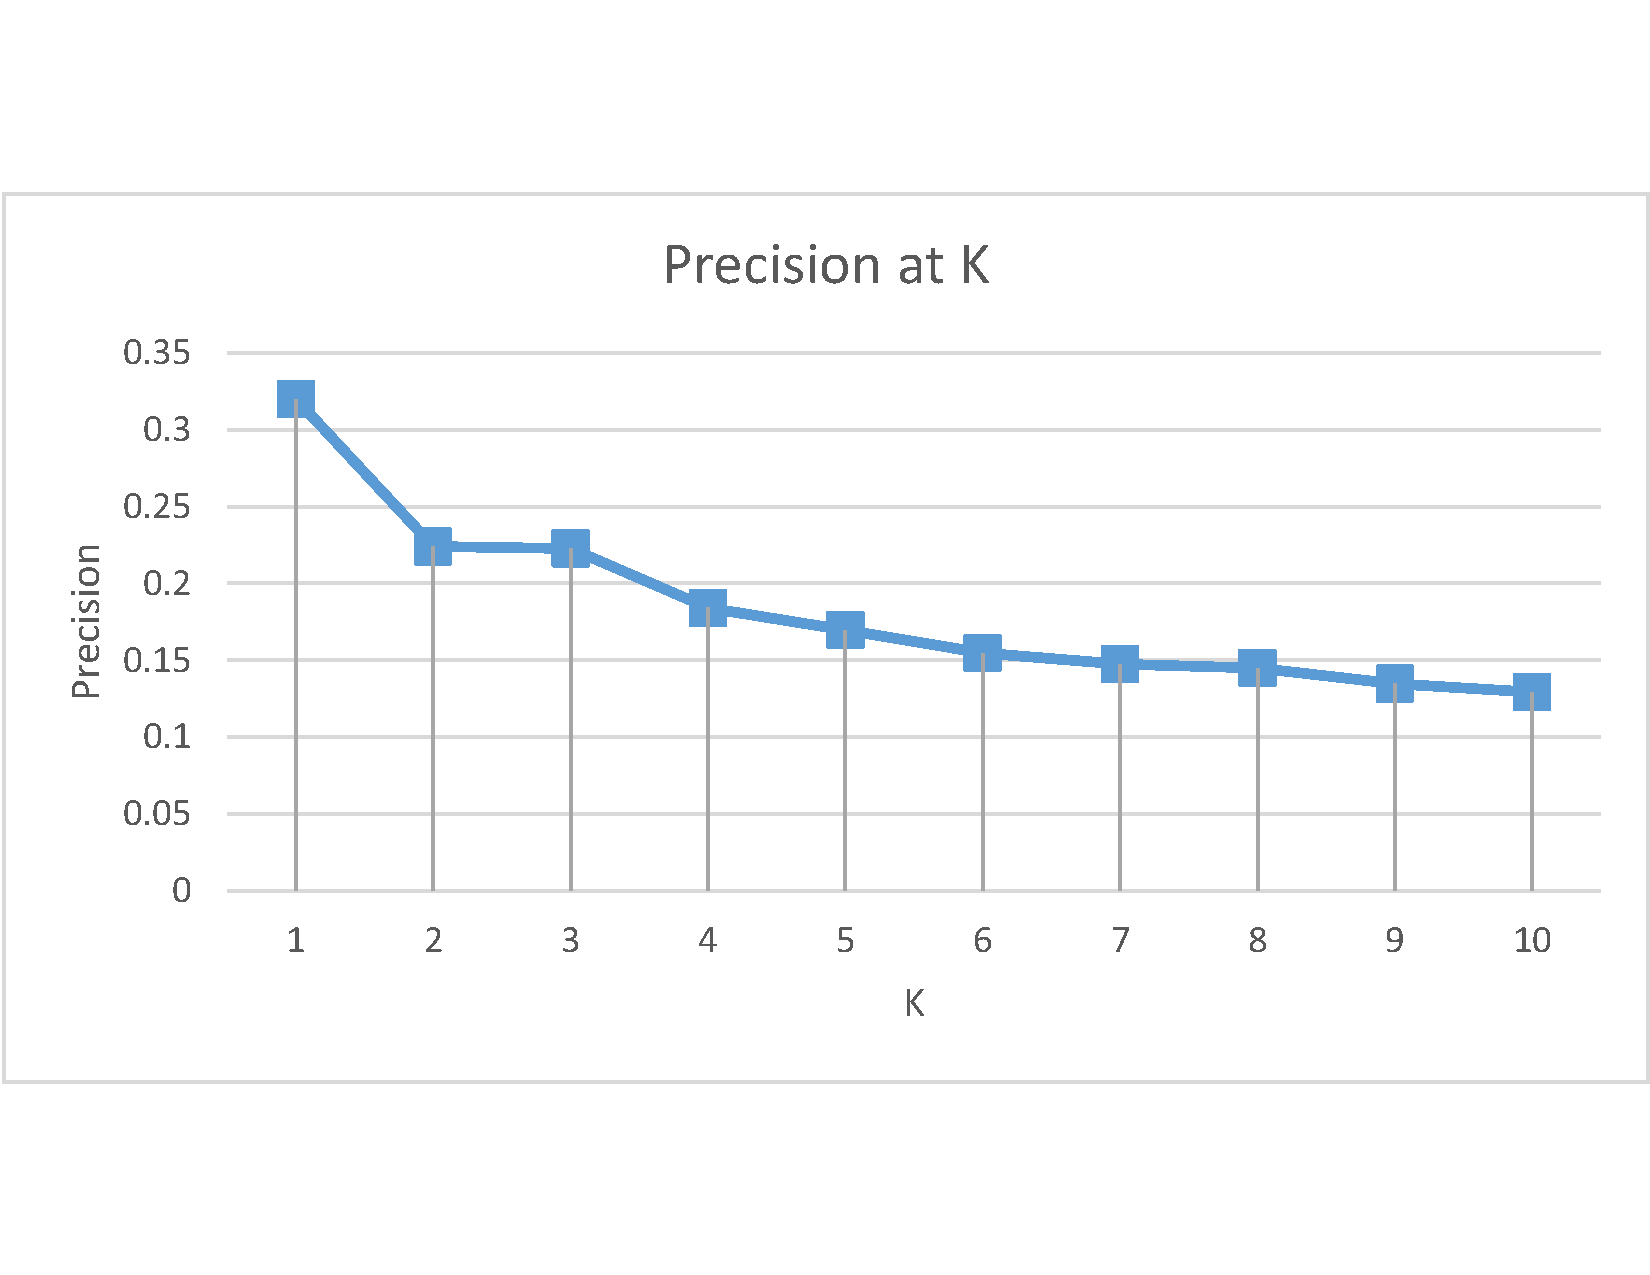
\includegraphics[width=\linewidth]{img/patk.pdf}
 \caption{Precision at K for action-noun map evaluation}
\end{figure}

\begin{table*}[th]
    \centering
    \caption{ Some of the results in Action-noun map we use for evaluation  }
    \begin{tabular} {|c|p{2cm}|p{2cm}|p{2cm}|p{2cm}|p{2cm}|}
    \hline
    Action class & \multicolumn{5}{c|}{Top 5 noun concepts from Action-noun map} \\
    \hline \hline
    event destroy place & disaster & wildfire & accident & threat & loss \\
    \hline
    group owe money & bankruptcy & billing & movie & trade & growth \\
    \hline
    group purchase item & acquisition & purchase & commerce & reporting & bankruptcy\\
    \hline
    person cook food & cooking & breakfast & meal & fair & holiday\\
    \hline
    person celebrate event &  celebration & birthday & holiday & function & dance\\
    \hline
    person enjoy issue &  hobby & athletics & entertainment & medium & lesson\\
    \hline
    person catch fish &  hobby & refreshment & fishing & drink & rodeo\\
    \hline
    brand sell product & update & hobby & entertainment & function & lesson\\
    \hline
    person assault group & assault & bar & practice & strike & killing\\
    \hline
    disease affect area &  illness & disease & threat & infection & anniversary\\
    \hline
    \end{tabular}
\end{table*}

\subsection{News search engine evaluation}
In order to evaluate the performance of our search engine, we have to prepare some evaluation data. Since our system's goal is
semantic search and retrieving the most relevant documents with respect to the query. We hope the evaluation data to contain
some implicit mentioning of searching query, for example the following piece of news is chosen from our evaluation data.

\begin{figure}[!htp]
 \centering
 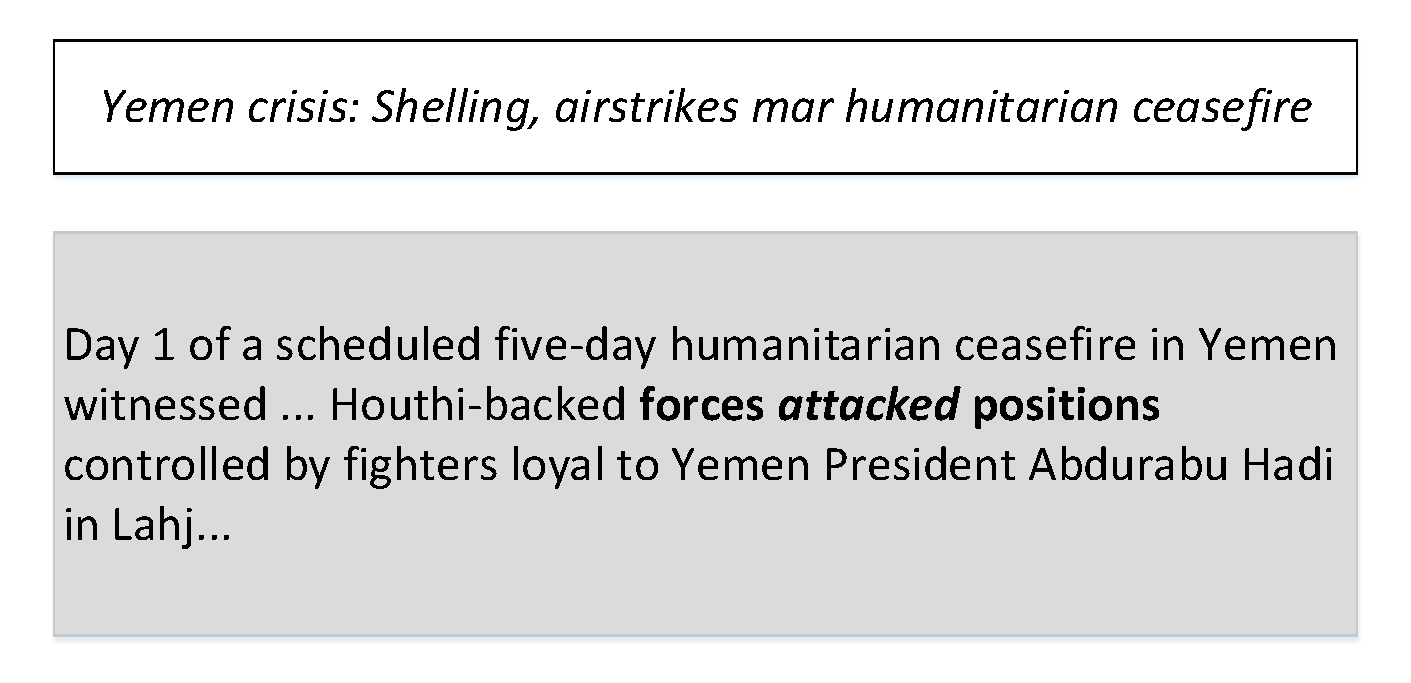
\includegraphics[width=\linewidth]{img/news.pdf}
\end{figure}


It is noticeable that this news is about ``war'', but there is no occurrence of the word ``war''. Hence we will have to
discover some actions, such as ``forces attacked positions'', to help us compute the relatedness between this news and ``war''.

Under the principal discussed above, We manually chose 10 queries based on the notion that those queries are likely to be mentioned
both explicitly and implicitly, then manually picked 10 positive documents and 10 negative documents
for each query in a news corpus of size 559,140, which is different from the news corpus we used to train our action-noun map
 to avoid bias towards our method.


The evaluation is intended to test if our action-based method would improve the searching quality, so we also implemented
two baselines using TF-IDF based searching algorithm and Topic model based searching algorithm.

We use an open-source search server based on Lucene called ElasticSearch \footnote{\url{https://www.elastic.co/}} for building our search engine system. The default retrieval algorithm of ElasticSearch
is based on TF-IDF, which calculates the term frequency of the query term in each document in our database, then by multiplying the
inverse document frequency of the query term, each document will be assigned a score representing the relatedness of this document with the
search query. Finally the documents are ranked according to the descending order of this score.

TF-IDF is a trivial baseline, apart from it we also implemented a Topic model baseline which uses Latent Dirichlet Allocation as enabling
technique. To build the LDA model we have to first train the word distribution for latent topics on a separate dataset. Here we use
a news corpus with around 497,299 unique news articles. We set the topic number to be 100 as an example and trained the model.
The result of the training phase will produce 1). The word distribution for each topic $P(word | topic)$ 2). The topic
distribution for a given document $P(topic | document)$.
The LDA model is then applied on each testing documents and as a result yields the topic distribution for each testing document.
During searching, the user query is first compared with word distribution, and we will be able to rank the topic according to $P(word | topic)$. Our idea is by $P(word | document) = P(word | topic) \times P(topic | document)$ we could rank the news documents.

In our system, we use a more complicated scoring function. Given a query consisting of several tokens \emph{$w_1$ $w_2$ ... $w_n$}, we score the j-th topic $t_j$ in the following way:

\begin{align}
    & S_{t_j, w_1, w_2 ... w_n} =   \sum_{i=1}^n TF_{ij} \times IDF_i \\
    & = \sum_{i=1}^n \frac{freq_{j}(w_i)}{\max \limits_{w \in WD_j} freq_{j}(w) } \times \log_{2}\frac{K}{n_i} \\
    & = \sum_{i=1}^n  \frac{P(w_i|t_j)}{\max \limits_{w \in WD_j}P(w|t_j)} \times \log_{2}\frac{K}{n_i}
  \end{align}

If we view a topic as a document, we can calculate the TF-IDF by taking the word frequency, or $P(word|topic)$ as TF and by counting the number of topics contain the word. Here $freq_{j}(w_i)$ is the frequency of word $w_i$ in topic $t_j$, $WD_j$ is the set of tokens in the word distribution of topic $t_j$,  $P(w_i|t_j)$ is the probability of generating the word $w_i$ when $t_j$ is picked to be the topic for this word, $K$ is the number of topics in LDA model and $n_i$ is the number of topics containing word $w_i$.

Finally by $S_{document,query} = S_{t_j, w_1, w_2 ... w_n} \times P(topic | document)$ we rank the news documents for the query.

In our method, we use the action-noun map generated previously, and first extract the action concepts in the testing dataset,
by applying our action-noun map on them we will get the noun equivalent for those action concepts. We add these noun concepts as
tags to the news documents representing the semantic abstraction of action concepts mentioned. During the index of the dataset we also
build a separate index for those noun tags. When user enters a query term, it will both compute TF-IDF results as in baseline and
an additional score for these noun tags. The final score is a linear combination of these two.
\begin{align}
Score(q, d) = W_0 \times Score(q, ac) + W_1 \times \text{TF-IDF}(q, d)
\end{align}
Where $q$ stands for query term. $d$ stands for document and $ac$ stands for the action noun concept representing the document. In our experiment, we choose $\text{TF-IDF}(q, collection of noun tags)$ as $Score(q, ac)$.
When we evaluate the news search engine.

\begin{table*}[th]
\centering
\caption{Evaluation Result on MRR and F1}
\begin{threeparttable}[b]
  \begin{tabular}{ c | p{1.7cm} | c | c | p{1.7cm} | c | c | p{1.7cm} | c | c } \hline
  & \multicolumn{3}{c|}{Action-based} &  \multicolumn{3}{c|}{LDA} &  \multicolumn{3}{c}{TF-IDF based} \\
  \hline \hline
  Query & Rank of 1st Pos\tnote{1} & F1\tnote{2} & AP \tnote{3} & First positive rank & F1 & AP & First positive rank & F1 & AP\\ \hline
  acquisition & 1 & 0.5 & 0.675 & 1 & 0.5 & 0.556 & 2 & 0.3 & 0.459 \\ \hline
  crime       & 1 & 0.5 & 0.588 & 8 & 0.2 & 0.342 & 4 & 0.3 & 0.385\\ \hline
  disaster    & 2 & 0.4 & 0.483 & 5 & 0.3 & 0.376 & 11 & 0.0 & 0.331 \\ \hline
  disease     & 2 & 0.4 & 0.476 & 6 & 0.3 & 0.415 & 3 & 0.1 & 0.376 \\ \hline
  election    & 1 & 0.4 & 0.488 & 1 & 0.7 & 0.742 & 10 & 0.1 & 0.348 \\ \hline
  music       & 1 & 0.4 & 0.546 & 1 & 0.7 & 0.728 & 1 & 0.5 & 0.574\\ \hline
  science     & 1 & 0.5 & 0.562 & 5 & 0.1 & 0.344 & 8 & 0.2 & 0.338\\ \hline
  sports      & 1 & 0.7 & 0.736 & 1 & 0.5 & 0.670 & 10 & 0.1 & 0.343\\ \hline
  terrorism   & 2 & 0.5 & 0.490 & 2 & 0.3 & 0.423 & 11 & 0.0 & 0.331\\ \hline
  war         & 1 & 0.6 & 0.812 & 1 & 0.7 & 0.800 & 8 & 0.1 & 0.335 \\ \hline
  MRR         & \multicolumn{3}{c|}{0.85} & \multicolumn{3}{c|}{0.62} & \multicolumn{2}{c}{0.27} \\ \hline
  F1 Mean     & \multicolumn{3}{c|}{0.49} & \multicolumn{3}{c|}{0.43} & \multicolumn{2}{c}{0.17} \\ \hline
  F1 Variance     & \multicolumn{3}{c|}{0.010} & \multicolumn{3}{c|}{0.049} & \multicolumn{2}{c}{0.025} \\ \hline
  MAP &  \multicolumn{3}{c|}{0.586} & \multicolumn{3}{c|}{0.540} &\multicolumn{3}{c}{0.382} \\ \hline
  \end{tabular}
  \begin{tablenotes}
    \item [1] The rank of the first positive news document
    \item [2] Since in our evaluation we view top 10 ranked news as predicted positive, and the total news number is 20, so Precision and Recall are the same
    \item [3] Average precision
    \end{tablenotes}
      \end{threeparttable}
\end{table*}
